% Created 2023-04-11 Tue 22:50
% Intended LaTeX compiler: pdflatex
\documentclass[12pt]{article}

%%%% settings when exporting code %%%% 

\usepackage{listings}
\lstdefinestyle{code-small}{
backgroundcolor=\color{white}, % background color for the code block
basicstyle=\ttfamily\small, % font used to display the code
commentstyle=\color[rgb]{0.5,0,0.5}, % color used to display comments in the code
keywordstyle=\color{black}, % color used to highlight certain words in the code
numberstyle=\ttfamily\tiny\color{gray}, % color used to display the line numbers
rulecolor=\color{black}, % color of the frame
stringstyle=\color[rgb]{0,.5,0},  % color used to display strings in the code
breakatwhitespace=false, % sets if automatic breaks should only happen at whitespace
breaklines=true, % sets automatic line breaking
columns=fullflexible,
frame=single, % adds a frame around the code (non,leftline,topline,bottomline,lines,single,shadowbox)
keepspaces=true, % % keeps spaces in text, useful for keeping indentation of code
literate={~}{$\sim$}{1}, % symbol properly display via latex
numbers=none, % where to put the line-numbers; possible values are (none, left, right)
numbersep=10pt, % how far the line-numbers are from the code
showspaces=false,
showstringspaces=false,
stepnumber=1, % the step between two line-numbers. If it's 1, each line will be numbered
tabsize=1,
xleftmargin=0cm,
emph={anova,apply,class,coef,colnames,colNames,colSums,dim,dcast,for,ggplot,head,if,ifelse,is.na,lapply,list.files,library,logLik,melt,plot,require,rowSums,sapply,setcolorder,setkey,str,summary,tapply},
aboveskip = \medskipamount, % define the space above displayed listings.
belowskip = \medskipamount, % define the space above displayed listings.
lineskip = 0pt} % specifies additional space between lines in listings
\lstset{style=code-small}
%%%% packages %%%%%

\usepackage[utf8]{inputenc}
\usepackage[T1]{fontenc}
\usepackage{lmodern}
\usepackage{textcomp}
\usepackage{color}
\usepackage{graphicx}
\usepackage{grffile}
\usepackage{wrapfig}
\usepackage{rotating}
\usepackage{longtable}
\usepackage{multirow}
\usepackage{multicol}
\usepackage{changes}
\usepackage{pdflscape}
\usepackage{geometry}
\usepackage[normalem]{ulem}
\usepackage{amssymb}
\usepackage{amsmath}
\usepackage{amsfonts}
\usepackage{dsfont}
\usepackage{array}
\usepackage{ifthen}
\usepackage{hyperref}
\usepackage{natbib}
%\VignetteIndexEntry{overview}
%\VignetteEngine{R.rsp::tex}
%\VignetteKeyword{R}
\RequirePackage{fancyvrb}
\DefineVerbatimEnvironment{verbatim}{Verbatim}{fontsize=\small,formatcom = {\color[rgb]{0.5,0,0}}}
\geometry{a4paper, left=15mm, right=15mm}
\RequirePackage{colortbl} % arrayrulecolor to mix colors
\RequirePackage{setspace} % to modify the space between lines - incompatible with footnote in beamer
\usepackage{authblk} % enable several affiliations (clash with beamer)
\renewcommand{\baselinestretch}{1.1}
\geometry{top=1cm}
\usepackage{enumitem}
\RequirePackage{xspace} %
\newcommand\Rlogo{\textbf{\textsf{R}}\xspace} %
\RequirePackage{epstopdf} % to be able to convert .eps to .pdf image files
\author{Brice Ozenne}
\date{\today}
\title{Overview of the functionalities of the package lavaSearch2}
\hypersetup{
 colorlinks=true,
 pdfauthor={Brice Ozenne},
 pdftitle={Overview of the functionalities of the package lavaSearch2},
 pdfkeywords={},
 pdfsubject={},
 pdfcreator={Emacs 26.3 (Org mode 9.4.6)},
 pdflang={English}
 }
\begin{document}

\maketitle
Load \textbf{lavaSearch2} in the R session:
\lstset{language=r,label= ,caption= ,captionpos=b,numbers=none}
\begin{lstlisting}
library(lavaSearch2)
\end{lstlisting}

\section{Inference}
\label{sec:orgb046af1}
\subsection{Introductory example}
\label{sec:org0d7082d}
You may have noticed that for simple linear regression, the p-values
of the Wald tests from \texttt{lm}:
\lstset{language=r,label= ,caption= ,captionpos=b,numbers=none}
\begin{lstlisting}
## simulate data
mSim <- lvm(Y[1:1]~0.3*X1+0.2*X2)
set.seed(10)
df.data <- sim(mSim, 2e1)

## fit linear model
summary(lm(Y~X1+X2, data = df.data))$coef
\end{lstlisting}

\begin{verbatim}
             Estimate Std. Error   t value    Pr(>|t|)
(Intercept) 0.7967775  0.2506767 3.1785069 0.005495832
X1          0.1550938  0.2205080 0.7033477 0.491360483
X2          0.4581556  0.2196785 2.0855736 0.052401103
\end{verbatim}


differ from those obtained with the corresponding latent variable
model estimated by maximum likelihood:
\lstset{language=r,label= ,caption= ,captionpos=b,numbers=none}
\begin{lstlisting}
## fit latent variable model
m <- lvm(Y~X1+X2)
e <- estimate(m, data = df.data)

## extract Wald tests
summary(e)$coef
\end{lstlisting}

\begin{verbatim}
      Estimate Std. Error   Z-value      P-value
Y~X1 0.1550938  0.2032984 0.7628877 0.4455303456
Y~X2 0.4581556  0.2025335 2.2621221 0.0236898575
Y~~Y 0.5557910  0.1757566 3.1622777           NA
Y    0.7967775  0.2311125 3.4475747 0.0005656439
\end{verbatim}


For instance, the p-value for the effect of X2 is 0.024 in the latent
variable model and 0.052 in the linear regression. The discrepancy is
due to 2 corrections that \texttt{lm} applies in order to improve the control
of the type 1 error of the Wald tests:
\begin{itemize}
\item use of a Student \(t\)-distribution instead of a Gaussian
distribution (informally using a t-value instead of z-value).
\item use of an unbiased estimator of the residuals variance instead of
the ML-estimator.  \textbf{lavaSearch2} attempts to generalize these
\end{itemize}
corrections to models with correlated and heteroschedastic
measurements. In the case of a simple linear regression, Wald tests
obtained with \textbf{lavaSearch2} match almost exactly those of \texttt{lm}:
\lstset{language=r,label= ,caption= ,captionpos=b,numbers=none}
\begin{lstlisting}
summary2(e)$coef
\end{lstlisting}

\begin{verbatim}
      estimate        se statistic    df     p.value
Y    0.7967775 0.2506766 3.1785073 17.00 0.005495827
Y~X1 0.1550938 0.2205080 0.7033478 17.00 0.491360428
Y~X2 0.4581556 0.2196784 2.0855738 17.00 0.052401076
Y~~Y 0.6538716 0.2242761        NA  4.25          NA
\end{verbatim}

\subsection{How it works in a nutshell}
\label{sec:org9da7fb3}

When using \textbf{lava}, the p.values that are obtained from the summary
(Wald tests) rely on a Gaussian approximation and maximum likelihood
estimation. While being asymptotically valid, they usually do not
provide a very accurate control of the type 1 error rate in small
samples. Simulations have shown that the type 1 error rate tends to be
too large, i.e. the p.values are have a downward bias. \textbf{lavaSearch2}
provides two improvements:
\begin{itemize}
\item using a Student's \(t\)-distribution instead of a Gaussian
distribution to account for the uncertainty on the variance of the
coefficients. The degrees of freedom are estimated using Satterwaite
approximation, i.e. identifying the chi-squared distribution that
best fit the observed moments of the variance of the coefficients.
\item (partially) correcting for the first order bias in the ML estimates
of the variance parameters. This correction also affects the
standard error of the estimates.
\end{itemize}

\subsection{Single univariate Wald test}
\label{sec:org00a24b1}

We will illustrate the functionalities using a simulated dataset:
\lstset{language=r,label= ,caption= ,captionpos=b,numbers=none}
\begin{lstlisting}
## simulate data
mSim <- lvm(Y1~eta,Y2~eta,Y3~0.4+0.4*eta,Y4~0.6+0.6*eta,eta~0.5*X1+0.7*X2)
latent(mSim) <- ~eta
set.seed(12)
df.data <- sim(mSim, n = 3e1, latent = FALSE)

## display
head(df.data)
\end{lstlisting}

\begin{verbatim}
          Y1         Y2          Y3         Y4         X1         X2
1 -1.7606233  0.1264910  0.66442611  0.2579355  0.2523400 -1.5431527
2  3.0459417  2.4631929  0.00283511  2.1714802  0.6423143 -1.3206009
3 -2.1443162 -0.3318033  0.82253070  0.3008415 -0.3469361 -0.6758215
4 -2.5050328 -1.3878987 -0.10474850 -1.7814956 -0.5152632 -0.3670054
5 -2.5307249  0.3012422  1.22046986 -1.0195188  0.3981689 -0.5138722
6 -0.9521366  0.1669496 -0.21422548  1.5954456  0.9535572 -0.9592540
\end{verbatim}


We first fit the latent variable model using, as usual, the \texttt{estimate}
function:
\lstset{language=r,label= ,caption= ,captionpos=b,numbers=none}
\begin{lstlisting}
m <- lvm(c(Y1,Y2,Y3,Y4)~eta, eta~X1+X2)
e <- estimate(m, data = df.data)
\end{lstlisting}

We can extract the Wald tests based on the traditional approach using
\texttt{summary}:
\lstset{language=r,label= ,caption= ,captionpos=b,numbers=none}
\begin{lstlisting}
summary(e)$coef[c("Y2","Y3","Y2~eta","Y3~eta","eta~X1","eta~X2"), ]
\end{lstlisting}

\begin{verbatim}
        Estimate Std. Error   Z-value      P-value
Y2     0.2335412  0.2448593 0.9537775 0.3401962906
Y3     0.5114275  0.1785886 2.8637186 0.0041869974
Y2~eta 0.9192847  0.2621248 3.5070497 0.0004531045
Y3~eta 0.2626930  0.1558978 1.6850339 0.0919820326
eta~X1 0.5150072  0.2513393 2.0490515 0.0404570768
eta~X2 0.6212222  0.2118930 2.9317729 0.0033703310
\end{verbatim}


As explain at the begining of this section, \textbf{lavaSearch2} implements
two corrections that can be directly applied by calling the \texttt{summary2}
method:
\lstset{language=r,label= ,caption= ,captionpos=b,numbers=none}
\begin{lstlisting}
summary2(e)$coef[c("Y2","Y3","Y2~eta","Y3~eta","eta~X1","eta~X2"), ]
\end{lstlisting}

\begin{verbatim}
        estimate        se statistic        df     p.value
Y2     0.2335412 0.2518218 0.9274067 12.332567 0.371510180
Y3     0.5114275 0.1828716 2.7966475 24.693254 0.009851893
Y2~eta 0.9192847 0.2653220 3.4647887  3.518708 0.031533355
Y3~eta 0.2626930 0.1562776 1.6809386  5.953880 0.144155715
eta~X1 0.5150072 0.2642257 1.9491180 20.047646 0.065412240
eta~X2 0.6212222 0.2221293 2.7966698 27.739008 0.009272041
\end{verbatim}


To use the Satterthwaite correction alone, set the argument
  \texttt{ssc} to \texttt{FALSE}:

\lstset{language=r,label= ,caption= ,captionpos=b,numbers=none}
\begin{lstlisting}
summary2(e, ssc = FALSE)$coef[c("Y2","Y3","Y2~eta","Y3~eta","eta~X1","eta~X2"), ]
\end{lstlisting}

\begin{verbatim}
        estimate        se statistic        df     p.value
Y2     0.2335412 0.2448593 0.9537775 12.911877 0.357711941
Y3     0.5114275 0.1785886 2.8637186 25.780552 0.008210968
Y2~eta 0.9192847 0.2621248 3.5070497  3.674640 0.028396459
Y3~eta 0.2626930 0.1558978 1.6850339  6.222912 0.141185621
eta~X1 0.5150072 0.2513393 2.0490515 21.571210 0.052814794
eta~X2 0.6212222 0.2118930 2.9317729 30.370334 0.006351686
\end{verbatim}


When using the Satterthwaite correction alone, the standard error are
left unchanged compared to the original lava output. The only change
is how the p-values are computed, i.e. based on the quantiles of a
Student's \(t\)-distribution instead of a Gaussian distribution. 

To only use the bias correction, set the argument \texttt{df} to \texttt{FALSE}:
\lstset{language=r,label= ,caption= ,captionpos=b,numbers=none}
\begin{lstlisting}
summary2(e, df = FALSE)$coef[c("Y2","Y3","Y2~eta","Y3~eta","eta~X1","eta~X2"), ]
\end{lstlisting}

\begin{verbatim}
        estimate        se statistic  df      p.value
Y2     0.2335412 0.2518218 0.9274067 Inf 0.3537154044
Y3     0.5114275 0.1828716 2.7966475 Inf 0.0051635832
Y2~eta 0.9192847 0.2653220 3.4647887 Inf 0.0005306482
Y3~eta 0.2626930 0.1562776 1.6809386 Inf 0.0927748494
eta~X1 0.5150072 0.2642257 1.9491180 Inf 0.0512813393
eta~X2 0.6212222 0.2221293 2.7966698 Inf 0.0051632271
\end{verbatim}

\subsection{Saving computation time with \texttt{estimate2}}
\label{sec:orgaa5d2f3}
For each call to \texttt{summary2} the small sample size correction(s) will
be recalculated. However the calculation of the sample correction(s)
can be time consuming.
\lstset{language=r,label= ,caption= ,captionpos=b,numbers=none}
\begin{lstlisting}
system.time(
    res <- summary2(e, ssc = FALSE)
)
\end{lstlisting}

\begin{verbatim}
 user  system elapsed 
0.128   0.000   0.129
\end{verbatim}


In such a case one can pre-compute the main terms of the correction
(e.g. the derivative of the variance-covariance matrix) once for all
using the \texttt{estimate2} method:
\lstset{language=r,label= ,caption= ,captionpos=b,numbers=none}
\begin{lstlisting}
e2 <- estimate2(e)
\end{lstlisting}

\texttt{estimate2} automatically store the pre-computed terms in the
\texttt{sCorrect} slot of the object. It also adds the class \texttt{lvmfit2} to the
object:
\lstset{language=r,label= ,caption= ,captionpos=b,numbers=none}
\begin{lstlisting}
class(e2)
\end{lstlisting}

\begin{verbatim}
[1] "lvmfit2" "lvmfit"
\end{verbatim}


Calling the  \texttt{summary} methods is now much faster:
\lstset{language=r,label= ,caption= ,captionpos=b,numbers=none}
\begin{lstlisting}
system.time(
    summary(e2)
)
\end{lstlisting}

\begin{verbatim}
 user  system elapsed 
0.027   0.000   0.026
\end{verbatim}

\subsection{Single multivariate Wald test}
\label{sec:org6c4b2cc}

The function \texttt{compare} from the lava package can be use to perform
multivariate Wald tests, i.e. to test simultaneously several linear
combinations of the coefficients. We can test the linear hypothesis by
specifying in \texttt{compare} the parameters we would like to test:
\lstset{language=r,label= ,caption= ,captionpos=b,numbers=none}
\begin{lstlisting}
resTest0 <- lava::compare(e, par = c("Y2","Y2~eta","eta~X1"))
resTest0
\end{lstlisting}

\begin{verbatim}

	- Wald test -

	Null Hypothesis:
	[Y2] = 0
	[Y2~eta] = 0
	[eta~X1] = 0

data:  
chisq = 21.332, df = 3, p-value = 8.981e-05
sample estimates:
          Estimate   Std.Err       2.5%     97.5%
[Y2]     0.2335412 0.2448593 -0.2463741 0.7134566
[Y2~eta] 0.9192847 0.2621248  0.4055295 1.4330399
[eta~X1] 0.5150072 0.2513393  0.0223912 1.0076231
\end{verbatim}

\texttt{compare} uses a chi-squared distribution to compute the p-values.
Similarly to the Gaussian approximation, while being valid
asymptotically this procedure may not provide a very accurate control
of the type 1 error rate in small samples. Fortunately, the correction
proposed for the univariate Wald statistic can be adapted to the
multivariate Wald statistic. This is achieved by \texttt{compare2}:
\lstset{language=r,label= ,caption= ,captionpos=b,numbers=none}
\begin{lstlisting}
resTest1 <- compare2(e, linfct = c("Y2","Y2~eta","eta~X1"))
resTest1
\end{lstlisting}

\begin{verbatim}

	- Wald test -

	Null Hypothesis:
	[Y2] = 0
	[Y2~eta] = 0
	[eta~X1] = 0

data:  
F-statistic = 6.7118, df1 = 3, df2 = 11.11, p-value = 0.007577
sample estimates:
          Estimate   Std.Err        df        2.5%     97.5%
[Y2]     0.2335412 0.2518218 12.332567 -0.31349486 0.7805774
[Y2~eta] 0.9192847 0.2653220  3.518708  0.14114161 1.6974278
[eta~X1] 0.5150072 0.2642257 20.047646 -0.03607414 1.0660884
\end{verbatim}

The same result could have been obtained by first defining a contrast
matrix to encode (by rows) which linear combination of coefficients
should be tested, e.g.:
\lstset{language=r,label= ,caption= ,captionpos=b,numbers=none}
\begin{lstlisting}
resC <- createContrast(e, linfct = c("Y2=0","Y2~eta=0","eta~X1=0"))
resC$contrast
\end{lstlisting}

\begin{verbatim}
             Y2 Y3 Y4 eta Y2~eta Y3~eta Y4~eta eta~X1 eta~X2 Y1~~Y1 Y2~~Y2 Y3~~Y3 Y4~~Y4
[Y2] = 0      1  0  0   0      0      0      0      0      0      0      0      0      0
[Y2~eta] = 0  0  0  0   0      1      0      0      0      0      0      0      0      0
[eta~X1] = 0  0  0  0   0      0      0      0      1      0      0      0      0      0
             eta~~eta
[Y2] = 0            0
[Y2~eta] = 0        0
[eta~X1] = 0        0
\end{verbatim}


and passing it to the argument \texttt{linfct}:
\lstset{language=r,label= ,caption= ,captionpos=b,numbers=none}
\begin{lstlisting}
resTest2 <- compare2(e2, linfct = resC$contrast)
identical(resTest1,resTest2)
\end{lstlisting}

\begin{verbatim}
[1] TRUE
\end{verbatim}


Now a F-distribution is used to compute the p-values. As before on can
set the argument \texttt{ssc} to \texttt{FALSE} to use the Satterthwaite
approximation alone:
\lstset{language=r,label= ,caption= ,captionpos=b,numbers=none}
\begin{lstlisting}
resTest3 <- compare2(e, ssc = FALSE, linfct = resC$contrast)
resTest3
\end{lstlisting}

\begin{verbatim}

	- Wald test -

	Null Hypothesis:
	[Y2] = 0
	[Y2~eta] = 0
	[eta~X1] = 0

data:  
F-statistic = 7.1107, df1 = 3, df2 = 11.13, p-value = 0.006182
sample estimates:
          Estimate   Std.Err       df         2.5%     97.5%
[Y2]     0.2335412 0.2448593 12.91188 -0.295812256 0.7628948
[Y2~eta] 0.9192847 0.2621248  3.67464  0.165378080 1.6731913
[eta~X1] 0.5150072 0.2513393 21.57121 -0.006840023 1.0368543
\end{verbatim}

In this case the F-statistic of \texttt{compare2} is the same as the
chi-squared statistic of \texttt{compare} divided by the rank of the contrast matrix:
\lstset{language=r,label= ,caption= ,captionpos=b,numbers=none}
\begin{lstlisting}
resTest0$statistic/qr(resC$contrast)$rank
\end{lstlisting}

\begin{verbatim}
   chisq 
7.110689
\end{verbatim}

\subsection{Robust Wald tests}
\label{sec:orgf3ea70d}

When one does not want to assume normality distributed residuals,
robust standard error can be used instead of the model based standard
errors. They can be obtained by setting the argument \texttt{robust} to \texttt{TRUE}
when computing univariate Wald tests:
\lstset{language=r,label= ,caption= ,captionpos=b,numbers=none}
\begin{lstlisting}
summary2(e, robust = TRUE)$coef[c("Y2","Y3","Y2~eta","Y3~eta","eta~X1","eta~X2"), ]
\end{lstlisting}

\begin{verbatim}
        estimate robust SE statistic        df     p.value
Y2     0.2335412 0.2353245 0.9924222 12.332567 0.340064859
Y3     0.5114275 0.1897160 2.6957534 24.693254 0.012453535
Y2~eta 0.9192847 0.1791240 5.1321143  3.518708 0.009583913
Y3~eta 0.2626930 0.1365520 1.9237580  5.953880 0.103104593
eta~X1 0.5150072 0.2167580 2.3759546 20.047646 0.027583693
eta~X2 0.6212222 0.2036501 3.0504385 27.739008 0.004986632
\end{verbatim}


By default the degrees of freedom of the modeled based variance is
used. Degrees of freedom can be computed via a Satterthwaite
approximation using \texttt{lava.options(df.robust=2)}. However it is not
recommended as the resulting degrees of freedom showed a strange
behavior. Multivariate Wald test can be obtained in a similar way
using the \texttt{compare2} method:
\lstset{language=r,label= ,caption= ,captionpos=b,numbers=none}
\begin{lstlisting}
compare2(e2, linfct = c("Y2","Y2~eta","eta~X1"), robust = TRUE)
\end{lstlisting}

\begin{verbatim}

	- Wald test -

	Null Hypothesis:
	[Y2] = 0
	[Y2~eta] = 0
	[eta~X1] = 0

data:  
F-statistic = 12.526, df1 = 3, df2 = 8.41, p-value = 0.001832
sample estimates:
          Estimate robust SE        df        2.5%     97.5%
[Y2]     0.2335412 0.2353245 12.332567 -0.27765746 0.7447400
[Y2~eta] 0.9192847 0.1791240  3.518708  0.39394539 1.4446240
[eta~X1] 0.5150072 0.2167580 20.047646  0.06292679 0.9670875
\end{verbatim}

It may be surprising that the (corrected) robust standard errors are
(in this example) smaller than the (corrected) model-based one. This
is also the case for the uncorrected one:
\lstset{language=r,label= ,caption= ,captionpos=b,numbers=none}
\begin{lstlisting}
rbind(robust = diag(crossprod(iid(e))),
      model = diag(vcov(e)))
\end{lstlisting}

\begin{verbatim}
               Y2         Y3         Y4        eta     Y2~eta     Y3~eta     Y4~eta
robust 0.04777252 0.03325435 0.03886706 0.06011727 0.08590732 0.02179453 0.02981895
model  0.05995606 0.03189389 0.04644303 0.06132384 0.06870941 0.02430412 0.03715633
           eta~X1     eta~X2    Y1~~Y1    Y2~~Y2     Y3~~Y3     Y4~~Y4  eta~~eta
robust 0.05166005 0.05709393 0.2795272 0.1078948 0.03769614 0.06923165 0.3198022
model  0.06317144 0.04489865 0.1754744 0.1600112 0.05112998 0.10152642 0.2320190
\end{verbatim}


This may be explained by the fact the robust standard error tends to
be liberal in small samples (e.g. see Kauermann 2001, A Note on the
Efficiency of Sandwich Covariance Matrix Estimation ).

\subsection{Assessing the type 1 error of the testing procedure}
\label{sec:org2f34c32}

The function \texttt{calibrateType1} can be used to assess the type 1 error
of a Wald statistic on a specific example. This however assumes that
the estimated model is correctly specified. Let's make an example. For
this we simulate some data:
\lstset{language=r,label= ,caption= ,captionpos=b,numbers=none}
\begin{lstlisting}
set.seed(10)
m.generative <- lvm(Y ~ X1 + X2 + Gene)
categorical(m.generative, labels = c("ss","ll")) <- ~Gene
d <- lava::sim(m.generative, n = 50, latent = FALSE)
\end{lstlisting}

Let's now imagine that we want to analyze the relationship between
Y and Gene using the following dataset:
\lstset{language=r,label= ,caption= ,captionpos=b,numbers=none}
\begin{lstlisting}
head(d)
\end{lstlisting}

\begin{verbatim}
            Y         X1         X2 Gene
1 -1.14369572 -0.4006375 -0.7618043   ss
2 -0.09943370 -0.3345566  0.4193754   ss
3 -0.04331996  1.3679540 -1.0399434   ll
4  2.25017335  2.1377671  0.7115740   ss
5  0.16715138  0.5058193 -0.6332130   ss
6  1.73931135  0.7863424  0.5631747   ss
\end{verbatim}


For this we fit define a LVM:
\lstset{language=r,label= ,caption= ,captionpos=b,numbers=none}
\begin{lstlisting}
myModel <- lvm(Y ~ X1 + X2 + Gene)
\end{lstlisting}

and estimate the coefficients of the model using \texttt{estimate}:
\lstset{language=r,label= ,caption= ,captionpos=b,numbers=none}
\begin{lstlisting}
e <- estimate(myModel, data = d)
e
\end{lstlisting}

\begin{verbatim}
                    Estimate Std. Error  Z-value  P-value
Regressions:                                             
   Y~X1              1.02349    0.12017  8.51728   <1e-12
   Y~X2              0.91519    0.12380  7.39244   <1e-12
   Y~Genell          0.48035    0.23991  2.00224  0.04526
Intercepts:                                              
   Y                -0.11221    0.15773 -0.71141   0.4768
Residual Variances:                                      
   Y                 0.67073    0.13415  5.00000
\end{verbatim}


We can now use \texttt{calibrateType1} to perform a simulation study. We just
need to define the null hypotheses (i.e. which coefficients should be
set to 0 when generating the data) and the number of simulations:
\lstset{language=r,label= ,caption= ,captionpos=b,numbers=none}
\begin{lstlisting}
mySimulation <- calibrateType1(e, 
                               param = "Y~Genell",
                               n.rep = 50, 
                               trace = FALSE, seed = 10)
\end{lstlisting}

To save time we only make 50 simulations but much more are necessary
to really assess the type 1 error rate. Then we can use the \texttt{summary}
method to display the results:
\lstset{language=r,label= ,caption= ,captionpos=b,numbers=none}
\begin{lstlisting}
summary(mySimulation)
\end{lstlisting}

\begin{verbatim}
Estimated type 1 error rate [95% confidence interval]
sample size: 50 | number of simulations: 50
            link statistic correction type1error                  CI
 [Y~Genell] == 0      Wald       Gaus       0.12 [0.05492 ; 0.24242]
                                 Satt       0.10 [0.04224 ; 0.21869]
                                  SSC       0.08 [0.03035 ; 0.19456]
                           SSC + Satt       0.08 [0.03035 ; 0.19456]

Corrections: Gaus = Gaussian approximation 
             SSC  = small sample correction 
             Satt = Satterthwaite approximation
\end{verbatim}

\clearpage

\section{Adjustment for multiple comparisons}
\label{sec:org3132637}
\subsection{Univariate Wald test, single model}
\label{sec:orgc7110d9}

When performing multiple testing, adjustment for multiple comparisons
is necessary in order to control the type 1 error rate, i.e. to
provide interpretable p.values. The \textbf{multcomp} package enables to do
such adjustment when all tests comes from the same \texttt{lvmfit} object:
\lstset{language=r,label= ,caption= ,captionpos=b,numbers=none}
\begin{lstlisting}
## simulate data
mSim <- lvm(Y ~ 0.25 * X1 + 0.3 * X2 + 0.35 * X3 + 0.4 * X4 + 0.45 * X5 + 0.5 * X6)
set.seed(10)
df.data <- sim(mSim, n = 4e1)

## fit lvm
e.lvm <- estimate(lvm(Y ~ X1 + X2 + X3 + X4 + X5 + X6), data = df.data)
name.coef <- names(coef(e.lvm))
n.coef <- length(name.coef)

## Create contrast matrix
resC <- createContrast(e.lvm, linfct = paste0("Y~X",1:6), rowname.rhs = FALSE)
resC$contrast
\end{lstlisting}

\begin{verbatim}
       Y Y~X1 Y~X2 Y~X3 Y~X4 Y~X5 Y~X6 Y~~Y
[Y~X1] 0    1    0    0    0    0    0    0
[Y~X2] 0    0    1    0    0    0    0    0
[Y~X3] 0    0    0    1    0    0    0    0
[Y~X4] 0    0    0    0    1    0    0    0
[Y~X5] 0    0    0    0    0    1    0    0
[Y~X6] 0    0    0    0    0    0    1    0
\end{verbatim}


\lstset{language=r,label= ,caption= ,captionpos=b,numbers=none}
\begin{lstlisting}
e.glht <- multcomp::glht(e.lvm, linfct = resC$contrast, rhs = resC$null)
summary(e.glht)
\end{lstlisting}

\begin{verbatim}

	 Simultaneous Tests for General Linear Hypotheses

Fit: estimate.lvm(x = lvm(Y ~ X1 + X2 + X3 + X4 + X5 + X6), data = df.data)

Linear Hypotheses:
            Estimate Std. Error z value Pr(>|z|)   
[Y~X1] == 0   0.3270     0.1589   2.058  0.20725   
[Y~X2] == 0   0.4025     0.1596   2.523  0.06611 . 
[Y~X3] == 0   0.5072     0.1383   3.669  0.00144 **
[Y~X4] == 0   0.3161     0.1662   1.902  0.28582   
[Y~X5] == 0   0.3875     0.1498   2.586  0.05554 . 
[Y~X6] == 0   0.3758     0.1314   2.859  0.02482 * 
---
Signif. codes:  0 ‘***’ 0.001 ‘**’ 0.01 ‘*’ 0.05 ‘.’ 0.1 ‘ ’ 1
(Adjusted p values reported -- single-step method)
\end{verbatim}

Note that this correction relies on the Gaussian approximation. To use
small sample corrections implemented in \textbf{lavaSearch2}, just call
\texttt{glht2} instead of \texttt{glht}:
\lstset{language=r,label= ,caption= ,captionpos=b,numbers=none}
\begin{lstlisting}
e.glht2 <- glht2(e.lvm, linfct = resC$contrast, rhs = resC$null)
summary(e.glht2)
\end{lstlisting}

\begin{verbatim}

	 Simultaneous Tests for General Linear Hypotheses

Multiple Comparisons of Means (two sided tests) 

Fit: estimate.lvm(x = lvm(Y ~ X1 + X2 + X3 + X4 + X5 + X6), data = df.data)
Standard errors: Model-based

Linear Hypotheses:
             estimate        se        df     lower     upper statistic p.value  
[Y~X1] == 0  0.327006  0.174976 33.000000 -0.158914  0.812926    1.8689 0.32895  
[Y~X2] == 0  0.402533  0.175670 33.000000 -0.085313  0.890380    2.2914 0.14817  
[Y~X3] == 0  0.507242  0.152209 33.000000  0.084548  0.929937    3.3325 0.01232 *
[Y~X4] == 0  0.316099  0.182995 33.000000 -0.192089  0.824288    1.7274 0.41283  
[Y~X5] == 0  0.387459  0.164970 33.000000 -0.070673  0.845590    2.3487 0.13153  
[Y~X6] == 0  0.375763  0.144712 33.000000 -0.026113  0.777639    2.5966 0.07617 .
---
Signif. codes:  0 ‘***’ 0.001 ‘**’ 0.01 ‘*’ 0.05 ‘.’ 0.1 ‘ ’ 1
(CIs/p-values adjusted for multiple comparisons -- single step max-test) 
Error when computing the adjusted p-value by numerical integration: 0.00012125
\end{verbatim}

The single step method is the appropriate correction when one wants to
report the most significant p-value relative to a set of
hypotheses. If the second most significant p-value is also to be
reported then the method "free" is more efficient:
\lstset{language=r,label= ,caption= ,captionpos=b,numbers=none}
\begin{lstlisting}
summary(e.glht2, test = multcomp::adjusted("free"))
\end{lstlisting}

\begin{verbatim}

	 Simultaneous Tests for General Linear Hypotheses

Multiple Comparisons of Means (two sided tests) 

Fit: estimate.lvm(x = lvm(Y ~ X1 + X2 + X3 + X4 + X5 + X6), data = df.data)
Standard errors: Model-based

Linear Hypotheses:
            estimate       se       df statistic p.value  
[Y~X1] == 0  0.32701  0.17498 33.00000    1.8689 0.12911  
[Y~X2] == 0  0.40253  0.17567 33.00000    2.2914 0.09129 .
[Y~X3] == 0  0.50724  0.15221 33.00000    3.3325 0.01242 *
[Y~X4] == 0  0.31610  0.18299 33.00000    1.7274 0.12911  
[Y~X5] == 0  0.38746  0.16497 33.00000    2.3487 0.09129 .
[Y~X6] == 0  0.37576  0.14471 33.00000    2.5966 0.06451 .
---
Signif. codes:  0 ‘***’ 0.001 ‘**’ 0.01 ‘*’ 0.05 ‘.’ 0.1 ‘ ’ 1
(CIs/p-values adjusted for multiple comparisons -- step down max-test)
\end{verbatim}

See the book: "Multiple Comparisons Using R" by Frank Bretz, Torsten
Hothorn, and Peter Westfall (2011, CRC Press) for details about the
theory underlying the \textbf{multcomp} package.

\subsection{Univariate Wald test, multiple models}
\label{sec:org11c88f0}

Pipper et al. in "A Versatile Method for Confirmatory Evaluation of
the Effects of a Covariate in Multiple Models" (2012, Journal of the
Royal Statistical Society, Series C) developed a method to assess the
effect of an exposure on several outcomes when a different model is
fitted for each outcome. This method has been implemented in the \texttt{mmm}
function from the \textbf{multcomp} package for glm and Cox
models. \textbf{lavaSearch2} extends it to \texttt{lvm}. 

Let's consider an example where we wish to assess the treatment effect
on three outcomes X, Y, and Z. We have at hand three measurements
relative to outcome Z for each individual:
\lstset{language=r,label= ,caption= ,captionpos=b,numbers=none}
\begin{lstlisting}
mSim <- lvm(X ~ Age + 0.5*Treatment,
            Y ~ Gender + 0.25*Treatment,
            c(Z1,Z2,Z3) ~ eta, eta ~ 0.75*treatment,
            Age[40:5]~1)
latent(mSim) <- ~eta
categorical(mSim, labels = c("placebo","SSRI")) <- ~Treatment
categorical(mSim, labels = c("male","female")) <- ~Gender

n <- 5e1
set.seed(10)
df.data <- sim(mSim, n = n, latent = FALSE)
head(df.data)
\end{lstlisting}

\begin{verbatim}
         X      Age Treatment          Y Gender         Z1         Z2          Z3
1 39.12289 39.10415   placebo  0.6088958 female  1.8714112  2.2960633 -0.09326935
2 39.56766 39.25191      SSRI  1.0001325 female  0.9709943  0.6296226  1.31035910
3 41.68751 43.05884   placebo  2.1551047 female -1.1634011 -0.3332927 -1.30769267
4 44.68102 44.78019      SSRI  0.3852728 female -1.0305476  0.6678775  0.99780139
5 41.42559 41.13105   placebo -0.8666783   male -1.6342816 -0.8285492  1.20450488
6 42.64811 41.75832      SSRI -1.0710170 female -1.2198019 -1.9602130 -1.85472132
   treatment
1  1.1639675
2 -1.5233846
3 -2.5183351
4 -0.7075292
5 -0.2874329
6 -0.4353083
\end{verbatim}

We fit a model specific to each outcome:
\lstset{language=r,label= ,caption= ,captionpos=b,numbers=none}
\begin{lstlisting}
lvmX <- estimate(lvm(X ~ Age + Treatment), data = df.data)
lvmY <- estimate(lvm(Y ~ Gender + Treatment), data = df.data)
lvmZ <- estimate(lvm(c(Z1,Z2,Z3) ~ 1*eta, eta ~ -1 + Treatment), 
                 data = df.data)
\end{lstlisting}

and combine them into a list of \texttt{lvmfit} objects:
\lstset{language=r,label= ,caption= ,captionpos=b,numbers=none}
\begin{lstlisting}
mmm.lvm <- multcomp::mmm(X = lvmX, Y = lvmY, Z = lvmZ)
\end{lstlisting}

We can then call \texttt{glht2} to apply the small sample corrections,
generate a contrast matrix containing tests for all coefficient
related to the treatment, and collect the results:
\lstset{language=r,label= ,caption= ,captionpos=b,numbers=none}
\begin{lstlisting}
lvm.glht2 <- glht2(mmm.lvm, linfct = "TreatmentSSRI")
summary(lvm.glht2)
\end{lstlisting}

\begin{verbatim}

	 Simultaneous Tests for General Linear Hypotheses

Multiple Comparisons of Means (two sided tests) 

Linear Hypotheses:
                         estimate        se        df     lower     upper statistic
X: [TreatmentSSRI] == 0  0.466150  0.253280 47.000000 -0.154910  1.087209    1.8405
Y: [TreatmentSSRI] == 0 -0.542096  0.261321 47.000000 -1.182874  0.098682   -2.0744
Z: [TreatmentSSRI] == 0 -0.619822  0.440397 47.000000 -1.699707  0.460063   -1.4074
                        p.value
X: [TreatmentSSRI] == 0  0.1863
Y: [TreatmentSSRI] == 0  0.1165
Z: [TreatmentSSRI] == 0  0.3912
(CIs/p-values adjusted for multiple comparisons -- single step max-test) 
Error when computing the adjusted p-value by numerical integration: 0.00025692
\end{verbatim}

This can be compared to the unadjusted p.values:
\lstset{language=r,label= ,caption= ,captionpos=b,numbers=none}
\begin{lstlisting}
summary(lvm.glht2, test = multcomp::adjusted("none"))
\end{lstlisting}

\begin{verbatim}

	 Simultaneous Tests for General Linear Hypotheses

Multiple Comparisons of Means (two sided tests) 

Linear Hypotheses:
                         estimate        se        df     lower     upper statistic
X: [TreatmentSSRI] == 0  0.466150  0.253280 47.000000 -0.043383  0.975682    1.8405
Y: [TreatmentSSRI] == 0 -0.542096  0.261321 47.000000 -1.067807 -0.016385   -2.0744
Z: [TreatmentSSRI] == 0 -0.619822  0.440397 47.000000 -1.505787  0.266143   -1.4074
                        p.value  
X: [TreatmentSSRI] == 0 0.07202 .
Y: [TreatmentSSRI] == 0 0.04354 *
Z: [TreatmentSSRI] == 0 0.16588  
---
Signif. codes:  0 ‘***’ 0.001 ‘**’ 0.01 ‘*’ 0.05 ‘.’ 0.1 ‘ ’ 1
(CIs/p-values not adjusted for multiple comparisons)
\end{verbatim}

\clearpage 

\section{Model diagnostic}
\label{sec:orgc1e79df}
\subsection{Detection of local dependencies}
\label{sec:org439924f}

The \texttt{modelsearch} function of \textbf{lava} is a diagnostic tool for latent
variable models. It enables to search for local dependencies
(i.e. model misspecification) and add them to the model. Obviously it
is a data-driven procedure and its usefulness can be discussed,
especially in small samples:
\begin{itemize}
\item the procedure is instable, i.e. is likely to lead to two different
models when applied on two different dataset sampled from the same
generative model.
\item it is hard to define a meaningful significance threshold since
p-values should be adjusted for multiple comparisons and sequential
testing. However traditional methods like Bonferroni-Holm tend to
over corrected and therefore reduce the power of the procedure since
they assume that the test are independent.
\end{itemize}

The function \texttt{modelsearch2} in \textbf{lavaSearch2} partially solves the
second issue by adjusting the p-values for multiple testing. Let's see
an example:
\lstset{language=r,label= ,caption= ,captionpos=b,numbers=none}
\begin{lstlisting}
## simulate data
mSim <- lvm(c(y1,y2,y3)~u, u~x1+x2)
latent(mSim) <- ~u
covariance(mSim) <- y2~y3
transform(mSim, Id~u) <- function(x){1:NROW(x)}
set.seed(10)
df.data <- lava::sim(mSim, n = 125, latent = FALSE)
head(df.data)
\end{lstlisting}

\begin{verbatim}
          y1           y2         y3         x1         x2 Id
1  5.5071523  4.883752014  6.2928016  0.8694750  2.3991549  1
2 -0.6398644  0.025832617  0.5088030 -0.6800096 -0.0898721  2
3 -2.5835495 -2.616715027 -2.8982645  0.1732145 -0.8216484  3
4 -2.5312637 -2.518185427 -2.9015033 -0.1594380 -0.2869618  4
5  1.6346220 -0.001877577  0.3705181  0.7934994  0.1312789  5
6  0.4939972  1.759884014  1.5010499  1.6943505 -1.0620840  6
\end{verbatim}


\lstset{language=r,label= ,caption= ,captionpos=b,numbers=none}
\begin{lstlisting}
## fit model
m <- lvm(c(y1,y2,y3)~u, u~x1)
latent(m) <- ~u
addvar(m) <- ~x2 
e.lvm <- estimate(m, data = df.data)
\end{lstlisting}

\texttt{modelsearch2} can be used to sequentially apply the \texttt{modelsearch}
function with a given correction for the p.values:
\lstset{language=r,label= ,caption= ,captionpos=b,numbers=none}
\begin{lstlisting}
resScore <- modelsearch2(e.lvm, alpha = 0.1, trace = FALSE)
displayScore <- summary(resScore)
\end{lstlisting}

\begin{verbatim}
Sequential search for local dependence using the score statistic 
The variable selection procedure retained 2 variables:
    link statistic      p.value adjusted.p.value dp.Info selected nTests
1   u~x2 36.436487 1.577228e-09     5.008615e-08       1     TRUE     10
2 y2~~y3  6.912567 8.559203e-03     6.056378e-02       1     TRUE      9
3  y3~x1  3.136429 7.656125e-02     2.814343e-01       1    FALSE      8
Confidence level: 0.9 (two sided, adjustement: fastmax)
\end{verbatim}


This indeed matches the highest score statistic found by
\texttt{modelsearch}:
\lstset{language=r,label= ,caption= ,captionpos=b,numbers=none}
\begin{lstlisting}
resScore0 <- modelsearch(e.lvm, silent = TRUE)
c(statistic = sqrt(max(resScore0$test[,"Test Statistic"])), 
  p.value = min(resScore0$test[,"P-value"]))
\end{lstlisting}

\begin{verbatim}
   statistic      p.value 
6.036264e+00 1.577228e-09
\end{verbatim}


We can compare the adjustment using the max distribution to bonferroni:
\lstset{language=r,label= ,caption= ,captionpos=b,numbers=none}
\begin{lstlisting}
data.frame(link = displayScore$table[,"link"],
           none = displayScore$table[,"p.value"],
           bonferroni = displayScore$table[,"p.value"]*displayScore$table[1,"nTests"],
           max = displayScore$table[,"adjusted.p.value"])
\end{lstlisting}

\begin{verbatim}
    link         none   bonferroni          max
1   u~x2 1.577228e-09 1.577228e-08 5.008615e-08
2 y2~~y3 8.559203e-03 8.559203e-02 6.056378e-02
3  y3~x1 7.656125e-02 7.656125e-01 2.814343e-01
\end{verbatim}


In theory, the correction based on the max statistic should give a p
value that is smaller or equal than the p value adjusted using
Bonferroni. However for for very small p-values, the max-correction
can be numerically inaccurate and result in p-values that are slightly
larger. The evolution of the estimation of a given coefficient across
the sequential search can be displayed using \texttt{autoplot}:

\begin{center}
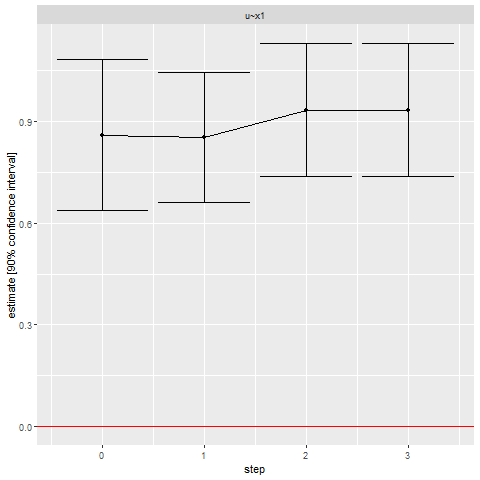
\includegraphics[width=.9\linewidth]{./modelsearch.png}
\end{center}

In many cases, all links are not plausible so the user should
indicates which links should be investigated by \texttt{modelsearch2}. This
can be done via the argument \texttt{link}:

\lstset{language=r,label= ,caption= ,captionpos=b,numbers=none}
\begin{lstlisting}
resRed <- modelsearch2(e.lvm, link = c("y1~~y2","y1~~y3","y2~~y3"), trace = FALSE)
print(resRed)
\end{lstlisting}

\begin{verbatim}
Sequential search for local dependence using the score statistic 
The variable selection procedure did not retain any variable 
    link statistic    p.value adjusted.p.value dp.Info selected nTests
1 y1~~y3  3.076875 0.07941299        0.1818963       1    FALSE      3
Confidence level: 0.95 (two sided, adjustement: fastmax)
\end{verbatim}


The function \texttt{findNewLink} can help the user to identify the set of
relevant links:
\lstset{language=r,label= ,caption= ,captionpos=b,numbers=none}
\begin{lstlisting}
findNewLink(e.lvm$model, type = "covariance")$link
\end{lstlisting}

\begin{verbatim}
[1] "y1~~y2" "y1~~y3" "y2~~y3"
\end{verbatim}

\subsection{Checking that the names of the variables in the model match those of the data}
\label{sec:org47cf06d}

When estimating latent variable models using \textbf{lava}, it sometimes
happens that the model does not converge:
\lstset{language=r,label= ,caption= ,captionpos=b,numbers=none}
\begin{lstlisting}
## simulate data
set.seed(10)
df.data <- sim(lvm(Y~X1+X2), 1e2)

## fit model
mWrong <- lvm(Y ~ X + X2)
eWrong <- estimate(mWrong, data = df.data)
\end{lstlisting}

\begin{verbatim}
Warning messages:
1: In estimate.lvm(mWrong, data = df.data) :
  Lack of convergence. Increase number of iteration or change starting values.
2: In sqrt(diag(asVar)) : NaNs produced
\end{verbatim}


This can have several reasons:
\begin{itemize}
\item the model is not identifiable.
\item the optimization routine did not managed to find a local
optimum. This may happen for complex latent variable model where the
objective function is not convex or locally convex.
\item the user has made a mistake when defining the model or has not given
the appropriate dataset.
\end{itemize}

The \texttt{checkData} function enables to check the last point. It compares
the observed variables defined in the model and the one given by the
dataset. In case of mismatch it returns a message:
\lstset{language=r,label= ,caption= ,captionpos=b,numbers=none}
\begin{lstlisting}
checkData(mWrong, df.data)
\end{lstlisting}

\begin{verbatim}
Missing variable in data: X
\end{verbatim}


In presence of latent variables, the user needs to explicitely define
them in the model, otherwise \texttt{checkData} will identify them as an
issue:
\lstset{language=r,label= ,caption= ,captionpos=b,numbers=none}
\begin{lstlisting}
## simulate data
set.seed(10)
mSim <- lvm(c(Y1,Y2,Y3)~eta)
latent(mSim) <- ~eta
df.data <- sim(mSim, n = 1e2, latent = FALSE)

## fit model
m <- lvm(c(Y1,Y2,Y3)~eta)
checkData(m, data = df.data)
\end{lstlisting}

\begin{verbatim}
Missing variable in data: eta
\end{verbatim}


\lstset{language=r,label= ,caption= ,captionpos=b,numbers=none}
\begin{lstlisting}
latent(m) <- ~eta
checkData(m, data = df.data)
\end{lstlisting}

\begin{verbatim}
No issue detected
\end{verbatim}



\clearpage

\section{Information about the R session used for this document}
\label{sec:org95dd3ad}

\lstset{language=r,label= ,caption= ,captionpos=b,numbers=none}
\begin{lstlisting}
sessionInfo()
\end{lstlisting}

\begin{verbatim}
R version 4.2.0 (2022-04-22)
Platform: x86_64-pc-linux-gnu (64-bit)
Running under: Ubuntu 20.04.4 LTS

Matrix products: default
BLAS:   /usr/lib/x86_64-linux-gnu/blas/libblas.so.3.9.0
LAPACK: /usr/lib/x86_64-linux-gnu/lapack/liblapack.so.3.9.0

locale:
 [1] LC_CTYPE=en_US.UTF-8       LC_NUMERIC=C               LC_TIME=en_US.UTF-8       
 [4] LC_COLLATE=en_US.UTF-8     LC_MONETARY=en_US.UTF-8    LC_MESSAGES=en_US.UTF-8   
 [7] LC_PAPER=en_US.UTF-8       LC_NAME=C                  LC_ADDRESS=C              
[10] LC_TELEPHONE=C             LC_MEASUREMENT=en_US.UTF-8 LC_IDENTIFICATION=C       

attached base packages:
[1] stats     graphics  grDevices utils     datasets  methods   base     

other attached packages:
[1] lavaSearch2_2.0.1 lava_1.7.2        ggplot2_3.4.0     butils.base_1.2  
[5] Rcpp_1.0.9        devtools_2.4.3    usethis_2.1.5     data.table_1.14.2

loaded via a namespace (and not attached):
 [1] pkgload_1.2.4            splines_4.2.0            foreach_1.5.2           
 [4] brio_1.1.3               assertthat_0.2.1         butils_1.4.7            
 [7] remotes_2.4.2            sessioninfo_1.2.2        globals_0.16.1          
[10] numDeriv_2016.8-1.1      pillar_1.8.1             lattice_0.20-45         
[13] glue_1.6.2               digest_0.6.31            colorspace_2.0-3        
[16] sandwich_3.0-2           Matrix_1.4-1             plyr_1.8.7              
[19] pkgconfig_2.0.3          listenv_0.8.0            purrr_1.0.0             
[22] mvtnorm_1.1-3            scales_1.2.1             processx_3.5.3          
[25] tibble_3.1.8             generics_0.1.3           ellipsis_0.3.2          
[28] TH.data_1.1-1            cachem_1.0.6             withr_2.5.0             
[31] cli_3.5.0                survival_3.5-0           magrittr_2.0.3          
[34] crayon_1.5.2             memoise_2.0.1            ps_1.7.0                
[37] fs_1.5.2                 future_1.28.0            fansi_1.0.3             
[40] parallelly_1.32.1        doParallel_1.0.17        nlme_3.1-157            
[43] MASS_7.3-57              xml2_1.3.3               RcppArmadillo_0.11.2.0.0
[46] pkgbuild_1.3.1           progressr_0.11.0         tools_4.2.0             
[49] prettyunits_1.1.1        lifecycle_1.0.3          multcomp_1.4-20         
[52] stringr_1.5.0            munsell_0.5.0            callr_3.7.0             
[55] compiler_4.2.0           rlang_1.0.6              grid_4.2.0              
[58] iterators_1.0.14         boot_1.3-28              testthat_3.1.4          
[61] gtable_0.3.1             codetools_0.2-18         abind_1.4-5             
[64] DBI_1.1.3                roxygen2_7.2.1           reshape2_1.4.4          
[67] R6_2.5.1                 zoo_1.8-11               knitr_1.39              
[70] dplyr_1.0.10             fastmap_1.1.0            future.apply_1.9.1      
[73] utf8_1.2.2               rprojroot_2.0.3          desc_1.4.1              
[76] stringi_1.7.8            parallel_4.2.0           vctrs_0.5.1             
[79] tidyselect_1.2.0         xfun_0.31
\end{verbatim}
\end{document}